This appendix shows several photos of the ultrapure water system in the same order that the water flows through them.

First of all, the complete scheme of the ultrapure water system is shown in Figure \ref{fig:SchemeUPWS}:

\begin{figure}[htbp]
\centering
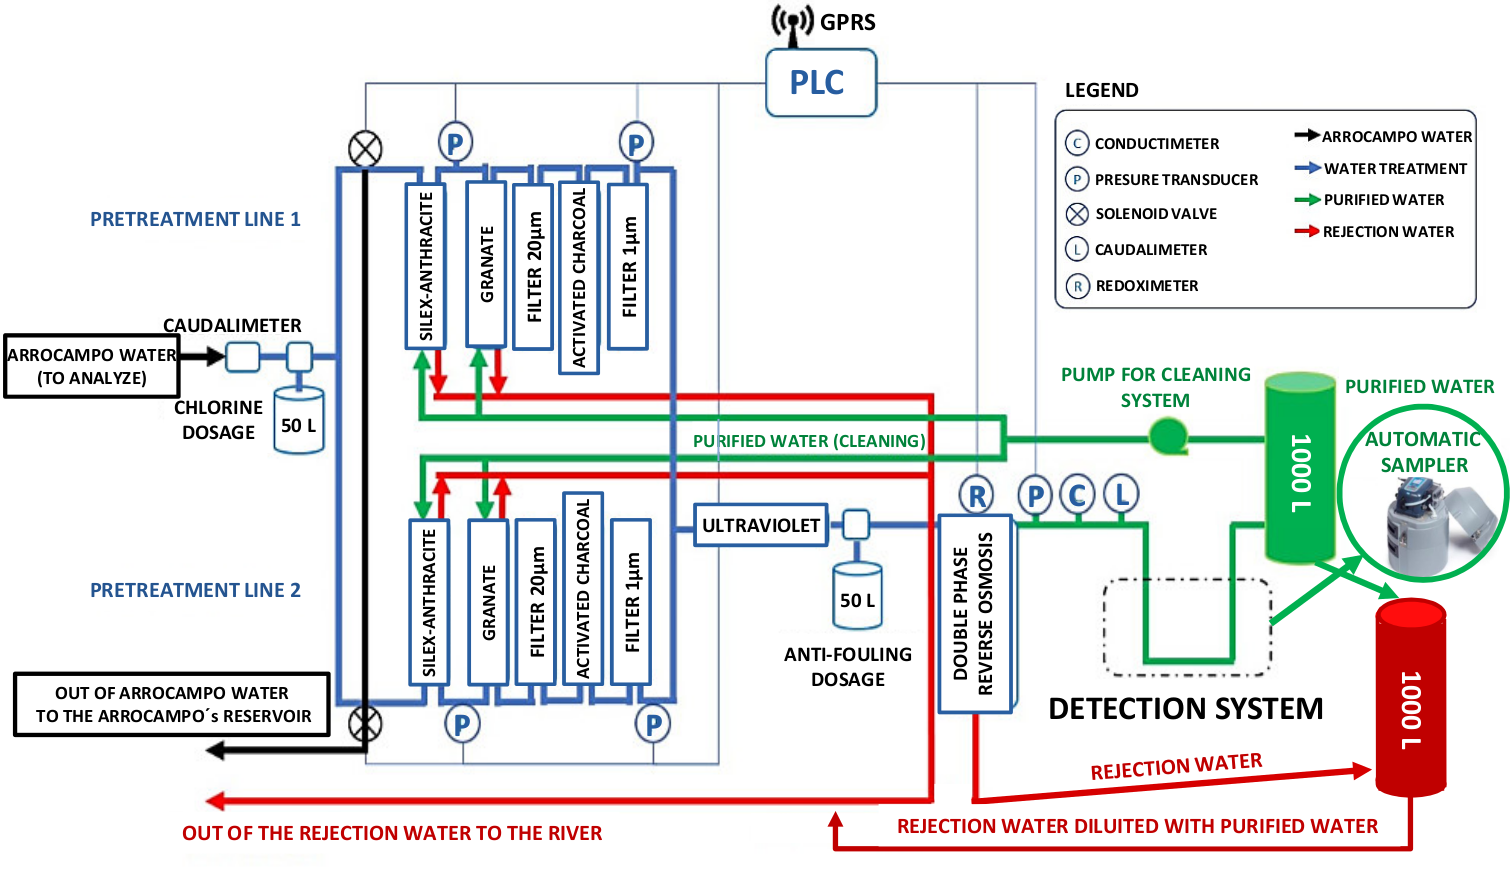
\includegraphics[scale=0.2]{9Appendix/93UltraPureWaterSystem/SchemeUltraPureWaterSystem.png}
\caption{Scheme of the ultrapure water system.\label{fig:SchemeUPWS}}
\end{figure}

The Gross filtering stage, made up of Silex-Antracite and Granate filters, the fine filtering stage, consisting of $20~\mu\meter$ filter and active carbon filter and the superfine filtering, composed of the $1~\mu\meter$ filter and the UV lamps, are shown in Figure \ref{fig:UltraPureWaterStages}.

\begin{figure}
\centering
    \begin{subfigure}[b]{0.3\textwidth}
    \centering
    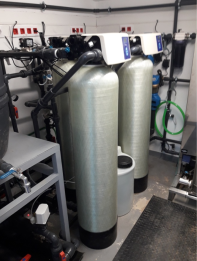
\includegraphics[width=\textwidth]{9Appendix/93UltraPureWaterSystem/GrossFiltering.png}  
    \caption{\label{subfig:GrossFiltering}}
    \end{subfigure}
    \hfill
    \begin{subfigure}[b]{0.3\textwidth}
    \centering
    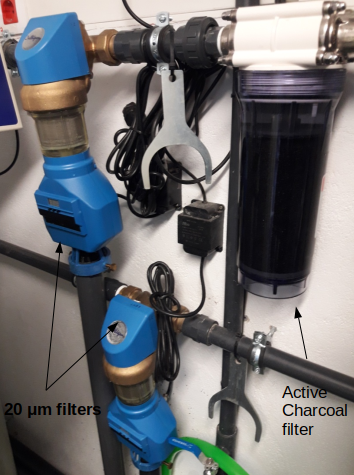
\includegraphics[width=\textwidth]{9Appendix/93UltraPureWaterSystem/FineFiltering.png}  
    \caption{\label{subfig:FineFiltering}}
    \end{subfigure}
    \hfill
    \begin{subfigure}[b]{0.3\textwidth}
    \centering
    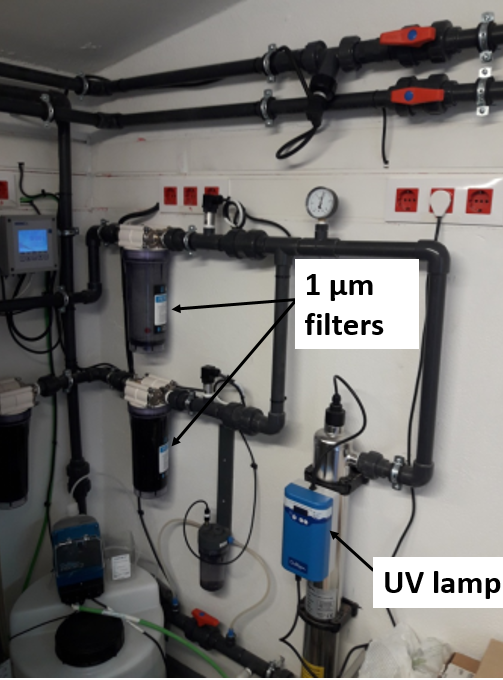
\includegraphics[width=\textwidth]{9Appendix/93UltraPureWaterSystem/SuperFineFiltering.png}  
    \caption{\label{subfig:SuperFineFiltering}}
    \end{subfigure}
 \caption{Different stages of filtration of the ultrapure water system. a) The gross filtering stage. b) The Fine filtering stage. c) The Super fine filtering stage.}
 \label{fig:UltraPureWaterStages}
\end{figure}

The double phase reverse osmosis is exhibited in Figure \ref{subfig:Osmosi} and the containers in which we store the ultrapure water and the reject water after treatment is displayed in Figure \ref{subfig:Containers}.

\begin{figure}
\centering
    \begin{subfigure}[b]{0.3\textwidth}
    \centering
    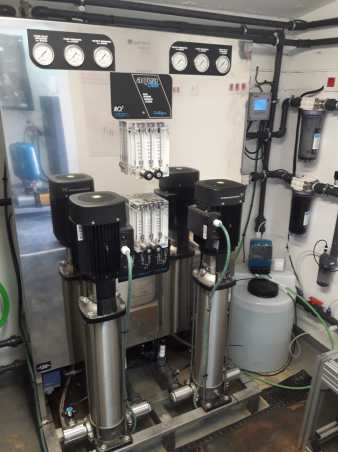
\includegraphics[width=\textwidth]{9Appendix/93UltraPureWaterSystem/Osmosi.png}  
    \caption{\label{subfig:Osmosi}}
    \end{subfigure}
    \hfill
    \begin{subfigure}[b]{0.5\textwidth}
    \centering
    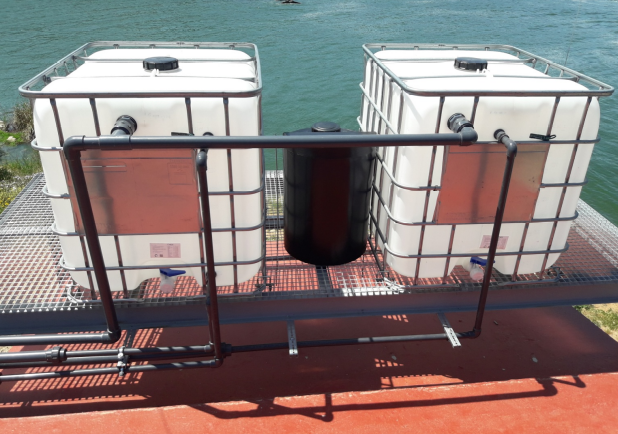
\includegraphics[width=\textwidth]{9Appendix/93UltraPureWaterSystem/Containers.png}  
    \caption{\label{subfig:Containers}}
    \end{subfigure}
 \caption{a) Doble phase reverse osmosis stage b) Containers used to store the outlet water of the ultrapure water system.}
 \label{subfig:OsmosisContainers}
\end{figure}

The Siemens PLC, software used to control the ultrapure water system, is shown in Figure \ref{fig:Siemens}.

\begin{figure}
\centering
    \begin{subfigure}[b]{0.37\textwidth}
    \centering
    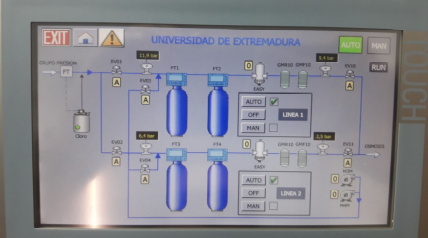
\includegraphics[width=\textwidth]{9Appendix/93UltraPureWaterSystem/Siemens1.png}  
    \caption{}
    \end{subfigure}
    \hfill
    \begin{subfigure}[b]{0.3\textwidth}
    \centering
    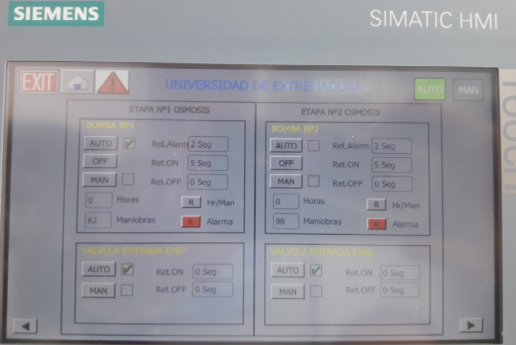
\includegraphics[width=\textwidth]{9Appendix/93UltraPureWaterSystem/Siemens2.png}  
    \caption{}
    \end{subfigure}
    \hfill
    \begin{subfigure}[b]{0.27\textwidth}
    \centering
    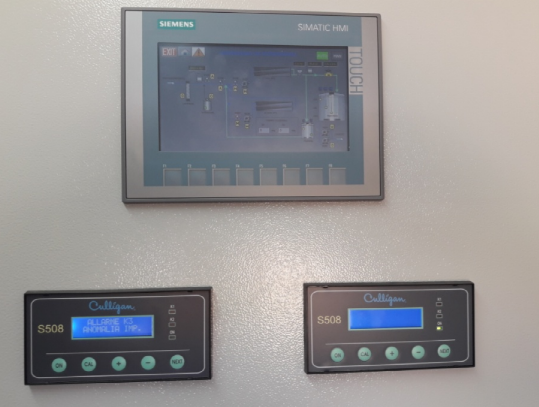
\includegraphics[width=\textwidth]{9Appendix/93UltraPureWaterSystem/Siemens3.png}  
    \caption{}
    \end{subfigure}
 \caption{Siemens PLC, software for remote control of ultrapure water system.}
 \label{fig:Siemens}
\end{figure}

Finally, the complete system of the ultrapure water system is displayed in Figure \ref{fig:CompleteSystem}

\begin{figure}[htbp]
\centering
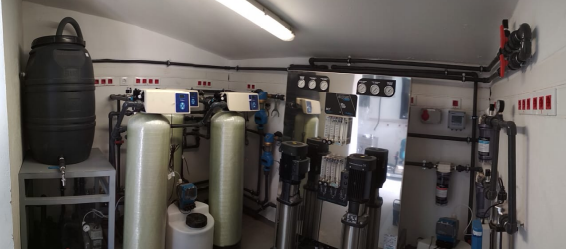
\includegraphics[scale=0.6]{9Appendix/93UltraPureWaterSystem/CompleteSystem.png}
\caption{General photo of the complete ultrapure water system.\label{fig:CompleteSystem}}
\end{figure}

Just as a curiosity, the three types of water (raw water, rejection water and ultrapure water) are exhibited in Figure \ref{fig:ThreeTypesOfWater}, where it can be visually checked the difference in the tubidity of each type of water.

\begin{figure}[htbp]
\centering
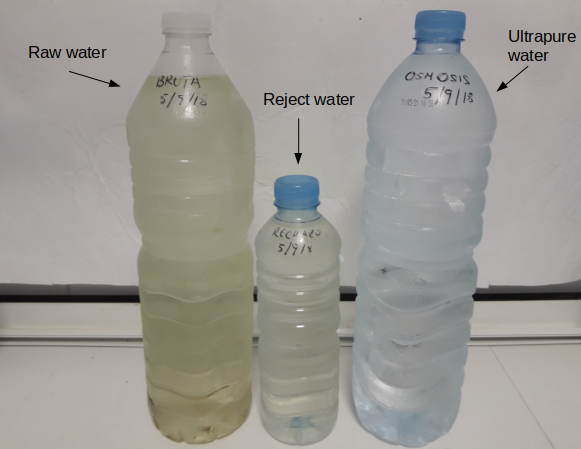
\includegraphics[scale=0.4]{9Appendix/93UltraPureWaterSystem/ThreeTypesOfWater.png}
\caption{Raw water, reject water and ultrapure water obtained with this system.\label{fig:ThreeTypesOfWater}}
\end{figure}
